\subsection{外观模式(Facade)}

\subsubsection{外观模式简介}

外观模式是一种设计模式,它允许一个类提供简单的接口来访问一个子系统中的一组类。这个模式为子系统中的一组复杂的类提供一个简单的接口,使得子系统更容易使用。

外观模式的主要用途是简化接口,减少客户端与子系统之间的依赖。这样,客户端可以更简单地使用子系统,而不必深入了解其内部工作原理。通过使用外观模式,可以让子系统的实现更容易扩展和更新,因为客户端的代码不会受到影响。

外观模式的优点包括:

\begin{enumerate}
    \item 简化了接口:通过提供一个统一的接口,外观模式可以简化访问子系统的接口,使得子系统更容易使用。
    \item 减少了客户端与子系统之间的依赖:外观模式可以隐藏子系统的内部工作原理,减少了客户端对子系统内部实现的依赖。
    \item 提高了系统的灵活性:通过使用外观模式,可以让子系统的实现更容易扩展和更新,因为客户端的代码不会受到影响。
\end{enumerate}

外观模式的缺点包括:

\begin{enumerate}
    \item 可能会过度抽象:如果外观模式的接口过于抽象,可能会导致客户端无法理解和使用它。
    \item 可能会增加系统的复杂度:如果外观模式过于复杂,可能会增加系统的复杂度,导致系统难以维护和扩展。
    \item 可能会掩盖子系统的问题:如果子系统存在问题,外观模式可能会掩盖这些问题,导致客户端无法及时发现并解决问题。
\end{enumerate}

\subsubsection{外观模式在项目中的应用}

\begin{figure}[H]
    \centering
    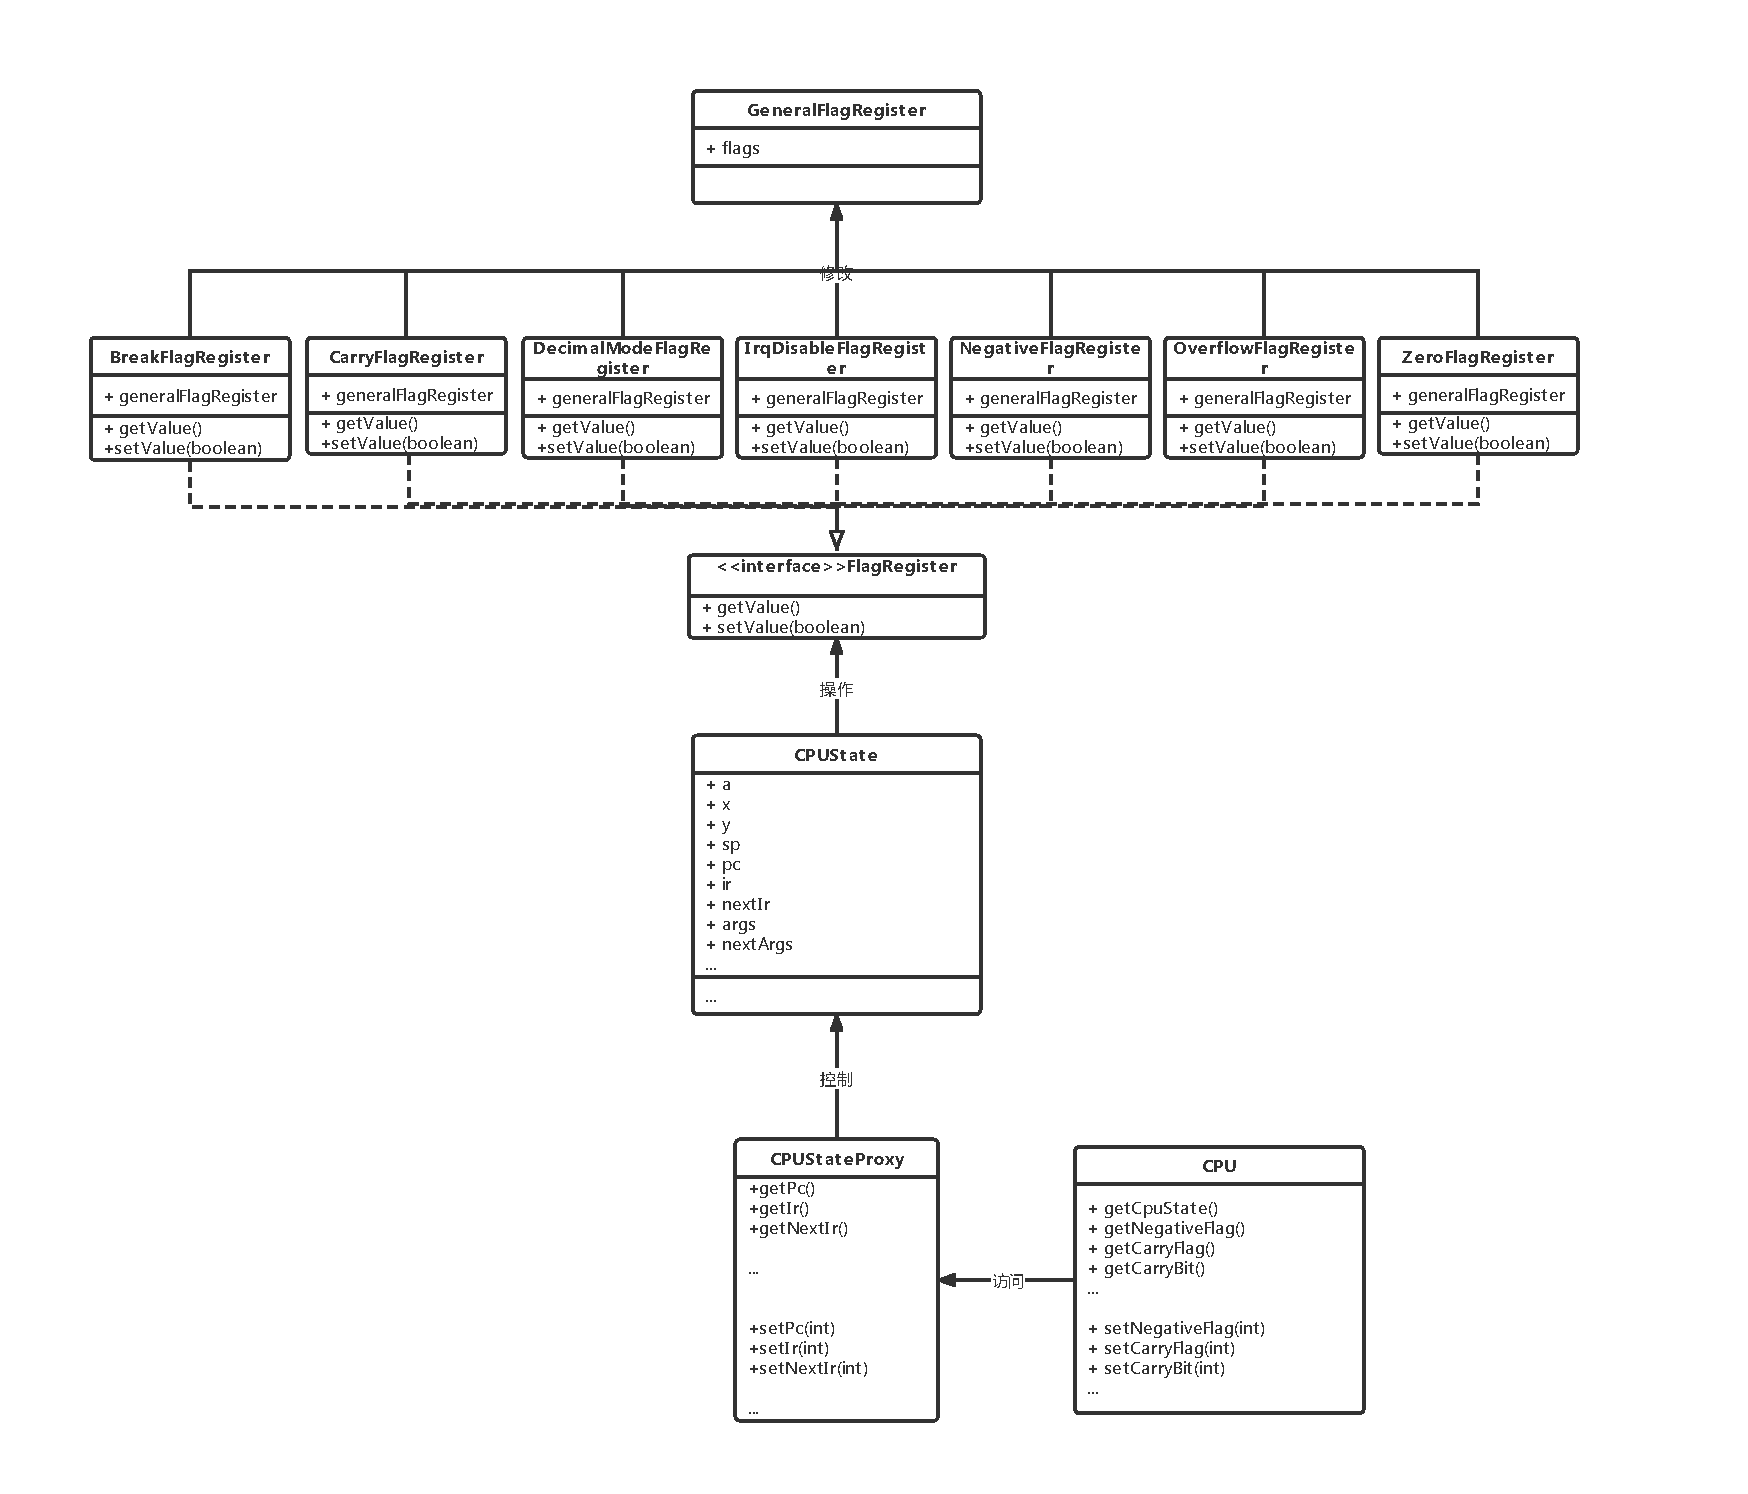
\includegraphics[width=0.9\textwidth]{figures/Facade.pdf}
    \caption{外观模式在 Slow6502 中的类图}
\end{figure}

本项目中,我们的 CPU State 类就是一个 Facade 。如果不使用这个 Facade ,那么各个寄存器的操作逻辑会被分散在 CPU 类中的各个部分。而使用了 Facade 模式之后,CPU 类可以使用 CPU State 提供简单的接口来访问一个子系统中的一组类,从而简化了逻辑,使其他类可以更简单地使用子系统,而不必深入了解其内部工作原理。